
\documentclass[11pt, a4paper]{article}

% --- Package essenziali ---
\usepackage[utf8]{inputenc}
\usepackage[T1]{fontenc}
\usepackage[english]{babel}
\usepackage{geometry}
\geometry{margin=2.5cm}

\usepackage{graphicx} % Grafica e figure
\usepackage{float} % Grafica e figure
\usepackage{booktabs} % Tabelle
\usepackage{array} % Tabelle
\usepackage{amsmath} % Matematica (utile per formule)
\usepackage[colorlinks=true, linkcolor=black, citecolor=blue, urlcolor=blue]{hyperref} % Hyperlinks nelle citazioni e nel PDF
\usepackage{graphicx}
\usepackage{subcaption}
%\usepackage{natbib} % Bibliografia
\usepackage{titling} % Linea orizzontale personalizzata
\usepackage[backend=biber,style=numeric,sorting=none]{biblatex} % Bibliografia
\addbibresource{bibliography.bib} % Bibliografia
% Codice/script nell'appendice
\usepackage{listings} 
\usepackage{xcolor}
\lstset{
    basicstyle=\ttfamily\small,
    breaklines=true,
    frame=single,
    backgroundcolor=\color{gray!10}
}


\begin{document}

% --- TITLE ---
{\centering
\footnotesize
Laboratory of Bioinformatics I \\
University of Bologna \\
Academic Year 2025--2026\par}




\noindent\rule{\textwidth}{0.4pt} % Linea sottile a tutta larghezza
%\vspace{6pt}

% Titolo e autore centrati
\begin{center}
    {\Large\textbf{Construction and validation of a profile hidden Markov model\\
    for the detection of the Kunitz domain}} \\[8pt]
    {\normalsize Valentina Rosemary Piccoli}
\end{center}

%\vspace{10pt}

% --- ABSTRACT ---
%\begin{abstract}
%    Your abstract here.
%\end{abstract}

% --- SECTION ---
\section{Introduction}
Sequence database homology searching is one of the most powerful tools in computational molecular biology, enabling the detection of remote 
evolutionary relationships between protein sequences. Among the probabilistic approaches developed for this purpose, Profile Hidden Markov 
Models (HMMs) have proven particularly effective for protein domain recognition. Unlike pairwise alignment tools such as BLAST, which rely on 
a context-independent substitution matrix, a profile HMM encodes position-specific amino acid frequencies and gap penalties derived from a 
multiple sequence alignment (MSA), capturing the evolutionary constraints characteristic of a specific protein family \cite{Eddy2011}. This 
position-specific scoring makes profile HMMs especially suited for detecting divergent or remote homologs that would be missed by simpler 
similarity searches.

The target of this work is the Kunitz domain (PFAM: PF00014), one of the most extensively studied protein domains in structural biology. The 
domain was first identified by \cite{Kunitz1936} in the bovine pancreatic trypsin inhibitor (BPTI), isolated from beef pancreas. Kunitz-domain 
inhibitors are found in animals, plants, and microbes \cite{Laskowski1980}, and are typically 50--70 amino acids in length. They adopt a 
conserved structural fold consisting of two antiparallel $\beta$-sheets and one or two helical regions, stabilized by three disulfide bridges 
with the bonding pattern C1--C6, C2--C4, C3--C5 \cite{Mishra2020}.
These disulfide bridges maintain the structural integrity of the inhibitor and present the protease-binding loop at the protein surface. 
A highly exposed P1 residue at position 15 (typically Arg or Lys) inserts into the S1 pocket of the target protease and is the primary 
determinant of inhibitory specificity \cite{Ascenzi2003}.

\begin{figure}[h]
    \centering
    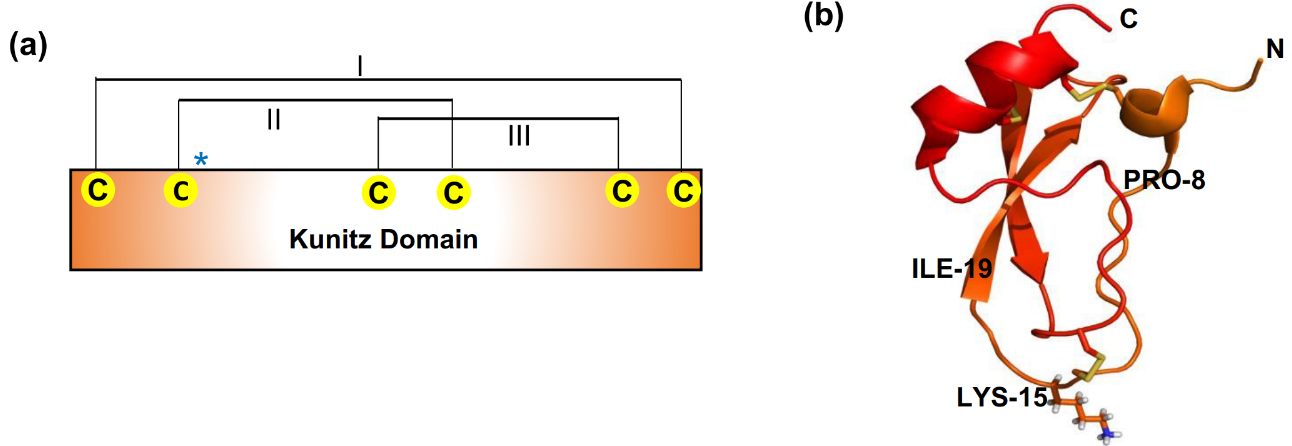
\includegraphics[width=\linewidth]{images/kunitz_domain.png}
    \caption{Structure and activity of Kunitz-domain inhibitors. (a) Schematic representation of Kunitz-domain inhibitor showing the disulfde 
    bonding pattern of 1-6, 2-4, 3-5. Conserved cysteine residues are marked with yellow and the P1 active site residue, the primary 
    determinant of the specifcity of serine protease inhibition is marked with a blue asterisk. (b) Crystal structure of BPTI (PDB: 4Y0Y) 
    showing three disulfde bonds (in yellow), the solvent-exposed loop (P8 to I19) highly complementary to the enzyme active site, and the P1 
    residue (K15).}
    \label{fig:kunitz_domain}
\end{figure}

%%%%%%%%%%%%%%%%%%%%%%%%%%%%%%%%%%%%%%%%%%%%%
\section{Materials and Methods}

\subsection{Dataset Construction}

Experimentally determined protein structures containing the Kunitz 
domain were retrieved from the RCSB Protein Data Bank 
(RCSB PDB) \cite{Burley2018} using the following search criteria: 
Annotation Identifier = ``PF00014'', Annotation Type = ``Pfam'', 
data collection resolution $\leq$ 3.5~\AA, and polymer entity 
sequence length between 40 and 70 amino acids. Results were 
downloaded in tabular format including the following fields: 
Entry ID, Sequence, Auth Asym ID, Entity ID, and Annotation 
Identifier. The initial query returned 134 PDB entries, 
corresponding to 6{,}229 rows in the tabular file (multiple rows 
per entry due to multiple annotation records per chain).

The tabular output was processed with a custom Python script. 
First, only rows with Annotation Identifier equal to ``PF00014'' 
were retained, in order to exclude co-crystallized chains that 
satisfied the resolution and length filters but did not carry 
the Kunitz domain annotation. This step was necessary because 
the PDB query returns all polymer entities of a structure when 
at least one entity satisfies the search criteria, including 
non-Kunitz co-crystallized partners.
A secondary sequence length filter (40–80 amino acids) was 
retained as a conservative criterion to exclude potential domain 
fragments (sequences shorter than 40 aa) and chains with extensive 
flanking regions (sequences longer than 80 aa). Three sequences 
were excluded by this filter: 5JBT:Y (38 aa, covering only positions 
323-360 of a Kunitz domain annotated at positions 306-364 in UniProt 
Q06481, suggesting an incomplete fragment), and 5NX1:C and 5NX3:C 
(81 aa each, both mapping to the Kunitz domain of APP, UniProt P05067, 
positions 289–346). The latter two sequences originate from the same 
protein as the training set structure 1AAP:A (also APP, UniProt P05067), 
which has a superior crystallographic resolution of 1.50 \AA compared to 
5NX1 (1.85 \AA) and 5NX3 (2.30 \AA). Consequently, 1AAP:A would have been 
selected as cluster representative regardless of whether 5NX1:C and 
5NX3:C were included, and their exclusion did not alter the final 
training set composition.
After filtering, 133 unique Kunitz domain chains were retained.

\subsection{Redundancy Removal}

The 133 chains were converted to FASTA format using a custom 
\texttt{awk} script. Sequence clustering was performed with 
MMseqs2 \cite{Steinegger2017} using a minimum sequence identity 
threshold of 0.8 and a minimum alignment coverage of 0.8.
These parameters were chosen for profile HMM construction, 
as a trade-off between redundancy reduction and 
preservation of sequence diversity. Clustering yielded 12 clusters.

The default MMseqs2 representative selection maximizes the number of sequences covered per cluster 
without considering crystallographic quality. Since the 
representative structures are subsequently used to build a 
multiple structure alignment, we implemented a custom Python 
script that selects, for each cluster, the structure with the 
lowest crystallographic resolution value (i.e., highest structural 
quality), querying resolution data via the RCSB PDB GraphQL API 
(\texttt{rcsb\_entry\_info.resolution\_combined} field). In the 
case of ties, the sequence with the greatest length was selected 
as tiebreaker. This procedure yielded 12 representative structures.

\subsection{Multiple Structure Alignment and Iterative Refinement}

The 12 representative PDB structures were downloaded from RCSB PDB 
and the chains of interest were extracted using a custom Python 
script, removing all co-crystallized molecules not corresponding 
to the Kunitz domain chain. Multiple structure alignment was 
performed with mTM-align \cite{Dong2018}.

An iterative refinement procedure was applied to improve the 
quality of the alignment, following two complementary criteria:

\textbf{RMSD-based criterion.} For each structure, the mean 
pairwise RMSD with respect to all other structures was computed 
from the mTM-align output matrix. Structures with a mean RMSD 
exceeding the global mean plus one standard deviation were 
considered outliers and removed. This conservative threshold 
(mean + 1 SD) was preferred over the simpler mean threshold to 
avoid over-removal of structures from an already small dataset.

\textbf{Cysteine alignment criterion.} The six conserved cysteine 
residues forming the three characteristic disulfide bridges of 
the Kunitz domain (pattern C1--C6, C2--C4, C3--C5) were used as 
structural anchors to evaluate alignment quality. Sequences with 
cysteine residues consistently misaligned with respect to the 
consensus positions were flagged for removal.

Additionally, manual inspection of the multiple sequence alignment 
derived from the multiple structure alignment revealed two pairs 
of nearly identical sequences originating from the same protein: 
3FP7\_J and 1G6X\_A (both Pancreatic trypsin inhibitor, UniProt 
P00974), and 5NX1\_D and 1AAP\_A (both Amyloid precursor protein, 
UniProt P05067). These pairs had not been merged by MMseqs2 because 
the shorter sequences (3FP7\_J and 5NX1\_D) exhibited an alignment 
coverage below the 0.8 threshold with respect to their longer 
counterparts. Redundancy was resolved manually by retaining the 
representative with the lowest crystallographic resolution and 
complete sequence coverage of all six cysteine residues, leading 
to the removal of 3FP7\_J and 5NX1\_D.

One sequence, 3WNY\_A, displayed an atypical cysteine pattern 
(only two cysteines aligned to positions C1 and C6 of the 
canonical motif). Despite this divergence, 3WNY\_A was retained 
because it carries a validated PF00014 annotation in UniProt, 
and its inclusion enriches the model with information about 
tolerated positional variability. Structure 4BQD\_A presented 
an N-terminal linker region (preceding the Kunitz domain as 
annotated in UniProt P10646) that did not align with any other 
sequence. This region was not removed manually, as it represents 
less than 50\% of any aligned column and is therefore treated 
as an insert state by \texttt{hmmbuild}, contributing no match 
states to the final model.

After the iterative refinement process, the final training set 
comprised 10 structures. The final multiple structure alignment 
yielded the following quality metrics: $L_\text{core}$ = 51, 
ccRMSD = 0.70~\AA, ccTM-score = 0.85, $L_\text{ali}$ = 55.04, 
RMSD = 0.84~\AA, TM-score = 0.90.

\subsection{HMM Model Construction}

The profile HMM was built from the multiple sequence alignment 
derived from the final multiple structure alignment using 
\texttt{hmmbuild} from the HMMER3 package \cite{Eddy2011} with 
default parameters. In the resulting model, alignment columns 
in which more than 50\% of sequences carry a gap are treated as 
insert states and do not contribute emission probabilities to the 
profile; the remaining columns become match states encoding 
position-specific amino acid frequencies.

\subsection{Validation Dataset}

Positive and negative sequence datasets were retrieved from the 
UniProt/Swiss-Prot database \cite{UniProt2023} (reviewed entries 
only), ensuring high annotation reliability. The positive set 
was defined by the query \texttt{(reviewed:true) AND 
(xref:pfam-PF00014)}, yielding sequences annotated with the 
Kunitz domain. The negative set was defined by 
\texttt{(reviewed:true) NOT (xref:pfam-PF00014)}, comprising 
all reviewed sequences lacking this annotation.

To avoid data leakage, the sequences corresponding to the 10 
structures used for model training were removed from the positive 
set. PDB chain identifiers were mapped to UniProt accession 
numbers using the UniProt ID Mapping tool, and the corresponding 
entries were excluded from the positive set using a custom Python 
script; removal was verified by confirming the absence of any 
overlap between training and positive set identifiers using the 
\texttt{comm} Unix utility. The final positive set comprised 390 
sequences. The negative set comprised 574{,}229 sequences, 
resulting in a heavily imbalanced dataset; the Matthews 
Correlation Coefficient (MCC) was therefore adopted as the 
primary performance metric, as it is robust to class imbalance 
unlike accuracy.

\subsection{Cross-Validation and Threshold Optimization}

Homology searches were performed with \texttt{hmmsearch} from 
HMMER3 \cite{Eddy2011} using the \texttt{--max} option to 
disable heuristic acceleration filters and maximize sensitivity, 
and \texttt{-Z 1000} to normalize the database size for 
comparable E-value computation across both datasets. The best 
domain E-value (column 8 of the \texttt{hmmsearch} tabular 
output) was used as the classification score in preference to 
the full-sequence E-value, as the Kunitz domain frequently 
occurs as an individual domain embedded within larger 
multidomain proteins; the domain-level score is therefore 
more informative for domain detection.

Sequences in the negative set that produced no match were 
assigned an E-value of 100 (substantially above the maximum 
observed E-value of 6.9) and labelled as true negatives. Both 
datasets were randomly shuffled prior to cross-validation 
(\texttt{sort -R}).

A two-fold cross-validation was performed by partitioning 
both the positive and negative sets into two equal folds, 
each containing 195 positive sequences and 287{,}115 negative 
sequences. In each iteration, one fold was used to optimize 
the E-value classification threshold and the complementary 
fold served as the validation set. Threshold optimization was 
performed by evaluating MCC over a grid of E-value thresholds 
ranging from $10^{-1}$ to $10^{-15}$. The optimal threshold 
was selected as the value yielding the highest MCC across 
both folds. A threshold of $10^{-5}$ was identified as optimal, 
producing consistent MCC values of 0.9923 on both folds.

%%%%%%%%%%%%%%%%%%%%%%%%%%%%%%%%%%%%%%%%%%%%%%%%%%%%%%
\section{Results}

\subsection{Training Set Composition}

Starting from 134 PDB entries retrieved by the initial query, 
the filtering pipeline retained 133 unique Kunitz domain chains. 
After clustering with MMseqs2 at 80\% sequence identity and 80\% 
coverage, 12 representative structures were selected based on 
crystallographic resolution. Table~\ref{tab:training} lists the 
10 structures constituting the final training set after the 
iterative MSA refinement process, together with their PDB 
identifiers, chain identifiers, source organisms, and 
crystallographic resolutions.

\begin{table}[H]
\centering
\caption{Final training set of 10 Kunitz domain structures.}
\label{tab:training}
\begin{tabular}{llll}
\toprule
PDB ID & Chain & Organism & Resolution (\AA) \\
\midrule
1AAP & A & \textit{Homo sapiens} & 1.50 \\
1G6X & A & \textit{Bos taurus} & 0.86 \\
1KTH & A & \textit{Homo sapiens} & 0.95 \\
1ZR0 & B & \textit{Homo sapiens} & 1.80 \\
3WNY & A & \textit{Bos taurus} & 1.30 \\
4BQD & A & \textit{Homo sapiens} & 2.48 \\
4DTG & K & \textit{Homo sapiens} & 1.80 \\
4ISO & B & \textit{Homo sapiens} & 2.10 \\
4U30 & X & \textit{Homo sapiens} & 2.50 \\
4U32 & X & \textit{Homo sapiens} & 1.65 \\
\bottomrule
\end{tabular}
\end{table}

The iterative refinement of the multiple structure alignment 
led to the removal of two sequences removed for manual 
redundancy resolution (3FP7\_J and 5NX1\_D). The final 
alignment of 10 structures achieved a TM-score of 0.90 and 
an RMSD of 0.84~\AA\ (Table~\ref{tab:msa_metrics}), 
reflecting the high structural conservation characteristic 
of the Kunitz domain fold.

\begin{table}[H]
\centering
\caption{Quality metrics of the final multiple structure 
alignment (mTM-align \cite{Dong2018}).}
\label{tab:msa_metrics}
\begin{tabular}{ll}
\toprule
Metric & Value \\
\midrule
$L_\text{core}$ & 51 \\
ccRMSD & 0.70~\AA \\
ccTM-score & 0.85 \\
$L_\text{ali}$ & 55.04 \\
RMSD & 0.84~\AA \\
TM-score & 0.90 \\
\bottomrule
\end{tabular}
\end{table}

\subsection{Model Performance}

The profile HMM was evaluated on both datatset folds 
(195 positive sequences and 287{,}115 or 287{},114 negative sequences) 
using the optimal E-value threshold of $10^{-5}$ identified 
by two-fold cross-validation. Figure~\ref{fig:mcc} shows the 
MCC as a function of the E-value threshold for both 
cross-validation folds, demonstrating consistent performance 
and a clear optimum at $10^{-5}$.

\begin{figure}
    \centering
    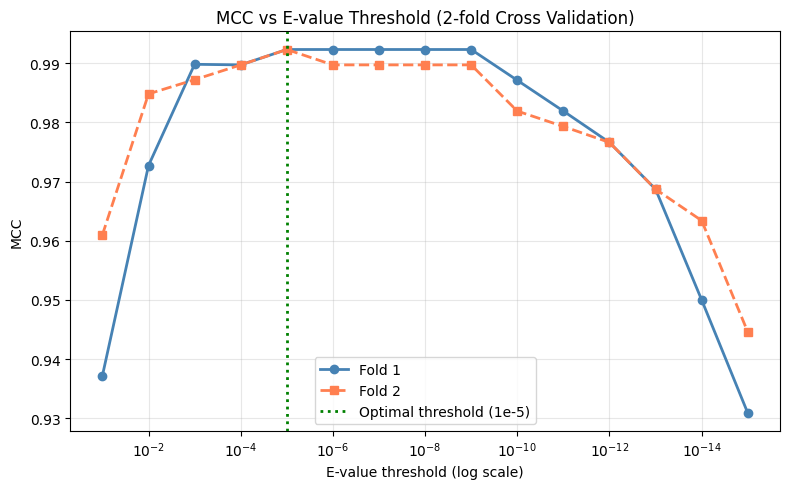
\includegraphics[width=\linewidth]{images/mcc_vc_eValue_threshold.png}
    \caption{}
    \label{fig:mcc}
\end{figure}

The confusion matrices for the two validation folds are 
reported in Figure~\ref{fig:cm}. 
The ROC curves for both folds are shown in 
Figure~\ref{fig:roc}, yielding AUC values close to 1.0, 
confirming the high discriminative power of the model 
across all possible threshold values.

\begin{figure}[H]
    \centering
    \begin{subfigure}[t]{0.45\textwidth}
        \centering
        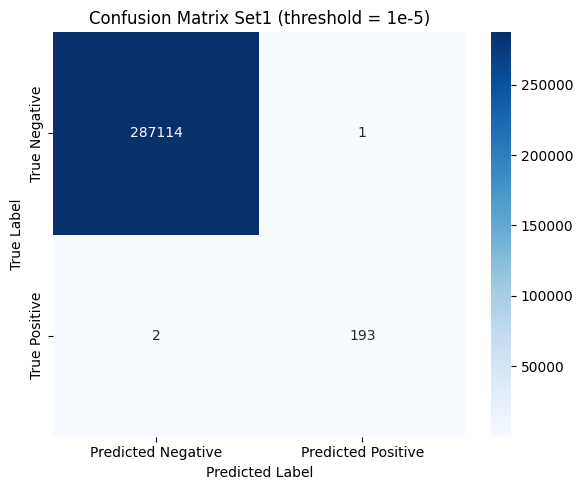
\includegraphics[width=\textwidth]{images/confusion_matrix_set1.png}
        \caption{}
    \end{subfigure}
    \hfill
    \begin{subfigure}[t]{0.45\textwidth} 
        \centering
        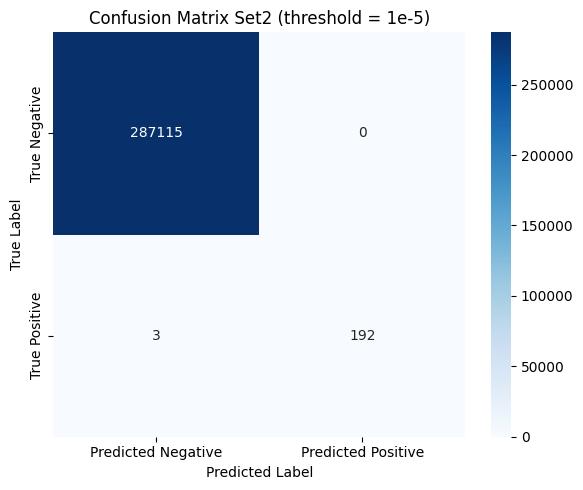
\includegraphics[width=\textwidth]{images/confusion_matrix_set2.png} 
        \caption{}
    \end{subfigure}
    \caption{Confusion matrices of both set1 (a) and set2 (b).}
    \label{fig:cm}
\end{figure}

\begin{figure}[H]
    \centering
    \begin{subfigure}[t]{0.45\textwidth}
        \centering
        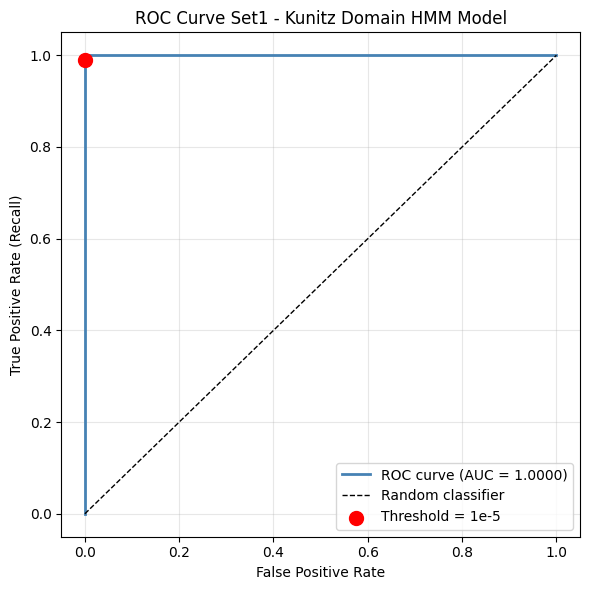
\includegraphics[width=\textwidth]{images/roc_curve_set1.png}
        \caption{}
    \end{subfigure}
    \hfill
    \begin{subfigure}[t]{0.45\textwidth} 
        \centering
        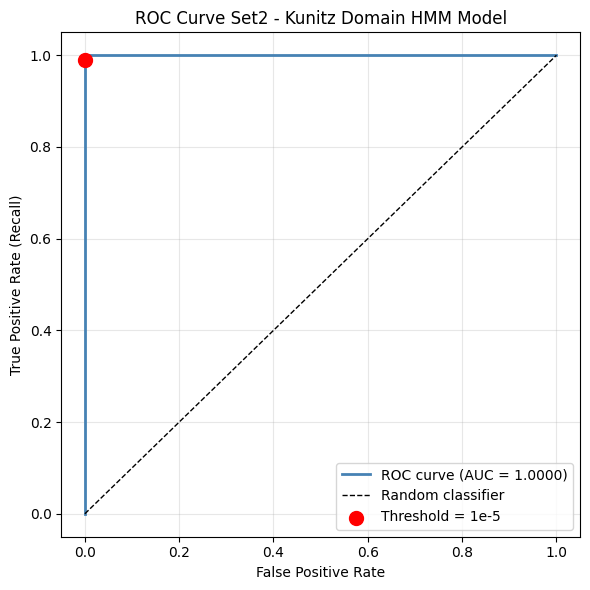
\includegraphics[width=\textwidth]{images/roc_curve_set2.png} 
        \caption{}
    \end{subfigure}
    \caption{ROC curves of both set1 (a) and set2 (b).}
    \label{fig:roc}
\end{figure}

\subsection{Analysis of False Negatives}

Five sequences annotated as Kunitz domain in UniProt were 
not detected by the model at the optimal threshold 
(Table~\ref{tab:fn}). All five carry computational 
annotations (PROSITE-ProRule PRU00031) rather than 
direct experimental evidence, introducing some uncertainty 
about their true classification status.

\begin{table}[H]
\centering
\caption{False negative sequences with best domain 
E-value and annotation evidence.}
\label{tab:fn}
\begin{tabular}{llrll}
\toprule
UniProt ID & Protein & E-value & \# Kunitz & Annotation \\
\midrule
Q8MVC4 & Penthalaris & $1.4 \times 10^{-5}$ & 5 & 
    PROSITE-ProRule \\
Q8WPG5 & Savignin & $2.1 \times 10^{-4}$ & 2 & 
    PROSITE-ProRule \\
A0A1Q1NL17 & HA11 & $8.7 \times 10^{-3}$ & 1 & 
    PROSITE-ProRule \\
O62247 & BLI-5 (\textit{C. elegans}) & $1.2 \times 10^{-2}$ & 
    1 & PROSITE-ProRule \\
D3GGZ8 & BLI-5 (\textit{H. contortus}) & $1.4 \times 10^{-1}$ 
    & 1 & PROSITE-ProRule \\
\bottomrule
\end{tabular}
\end{table}

Structural analysis using AlphaFold-predicted structures 
\cite{Jumper2021} confirmed that D3GGZ8 and O62247 are 
structurally divergent from the training set (pairwise RMSD 
of 1.55--1.85~\AA\ versus the training set average), yet 
highly similar to each other (RMSD = 0.35~\AA). Both 
sequences originate from nematodes (\textit{Haemonchus 
contortus} and \textit{Caenorhabditis elegans}), organisms 
evolutionarily distant from the vertebrates dominating the 
training set. Furthermore, both lack cysteines at positions 
C2 and C4, losing the central disulfide bridge (C2--C4) of 
the canonical pattern. The combination of high structural 
divergence, atypical cysteine pattern, and evolutionary 
distance suggests these sequences represent remote homologs 
of the Kunitz domain that are not well represented in the 
training set. An additional contributing factor is the 
position of the Kunitz domain within the full-length protein 
sequence: both D3GGZ8 and O62247 carry the domain at 
positions 120--190 and 135--184, respectively, within 
proteins of approximately 195--202 amino acids. The presence 
of flanking non-Kunitz sequence increases the effective 
length used for E-value computation, penalizing the 
domain-level score.

Q8WPG5 shows high structural divergence from the training 
set (RMSD = 2.1--2.7~\AA) despite a very high AlphaFold 
pLDDT score in the Kunitz domain region, suggesting a 
genuinely atypical fold rather than a prediction artifact. 
It lacks cysteine C4, disrupting the C2--C4 disulfide bridge.

Q8MVC4 represents a borderline case: with five Kunitz 
domains and a best domain E-value of $1.4 \times 10^{-5}$, 
it falls just above the optimal threshold of $10^{-5}$. 
A marginally more permissive threshold would correctly 
classify this sequence.

A0A1Q1NL17 shows intermediate divergence (RMSD = 
1.2--1.5~\AA) and lacks cysteine C2. Its relatively high 
E-value ($8.7 \times 10^{-3}$) likely reflects sequence 
divergence from the training set rather than a structural 
anomaly.

The single false positive was not investigated in detail 
given the very low false positive rate (1 out of 
574{,}229 negative sequences).


\section{Discussion and Conclusions}

In this work, a profile HMM for the detection of the Kunitz 
domain (PF00014) was constructed from a set of 10 
experimentally determined structures and evaluated on a 
large, curated sequence dataset from UniProt/Swiss-Prot. 
The model achieves an MCC of 0.9923, demonstrating high 
discriminative power despite the severe class imbalance 
between positive (390) and negative (574{,}229) sequences.

Several methodological choices contributed to the quality 
of the final model. First, the use of crystallographic 
resolution as the criterion for selecting cluster 
representatives, rather than the default 
approach of MMseqs2, ensured that the training structures 
provided the most reliable atomic coordinates for multiple 
structure alignment. Second, the combination of 
RMSD-based and cysteine-alignment criteria in the iterative 
refinement of the MSA allowed the removal of structurally 
inconsistent sequences while retaining legitimate variants 
such as 3WNY\_A, which displays an atypical cysteine 
pattern yet carries a validated Kunitz domain annotation. 
Third, the use of the best domain E-value rather than the 
full-sequence E-value for classification correctly accounts 
for the frequent occurrence of the Kunitz domain as an 
embedded domain within larger multidomain proteins.

An important observation emerging from the false negative 
analysis is the divergence between the RMSD-based outlier 
criterion and the cysteine alignment criterion during MSA 
refinement. These two criteria identified different 
candidate structures for removal, highlighting that 
structural divergence at the global level (RMSD) does not 
necessarily correspond to disruption of the functionally 
critical cysteine positions, and vice versa. This 
observation suggests that a combined evaluation is 
necessary for robust training set curation.

The five false negatives all carry computational 
annotations (PROSITE-ProRule PRU00031) rather than direct 
experimental evidence, and four of them display structural 
or sequence features suggesting divergence from canonical 
Kunitz domain members: atypical disulfide bridge patterns, 
evolutionary distance from the training set organisms, or 
domain positioning within long multidomain proteins. These 
findings suggest that the false negatives may represent 
remote homologs or divergent variants that are 
underrepresented in the training set, which was 
predominantly built from vertebrate structures.

Several limitations should be acknowledged. The training 
set comprises only 10 structures, predominantly from 
vertebrates, which may limit the model's sensitivity 
towards evolutionarily divergent Kunitz domain sequences 
from other taxa. Additionally, the clustering parameters 
(identity = coverage = 0.8) were fixed; exploring a range 
of values (0.8--0.95) could 
yield models with different sensitivity-specificity 
trade-offs. Future work should address these limitations 
by expanding the training set with structurally 
characterized Kunitz domains from non-vertebrate organisms 
and by performing a systematic evaluation across multiple 
clustering parameter settings.

In conclusion, the profile HMM constructed in this work 
accurately detects the Kunitz domain in Swiss-Prot reviewed 
sequences, with very few misclassifications. The 
methodological pipeline, from structure-guided training set 
curation to cross-validated threshold optimization, provides 
a reproducible framework applicable to the construction of 
profile HMMs for other protein domain families.

% --- BIBLIOGRAPHY---
\nocite{*} 
\printbibliography
%\bibliographystyle{plainnat}
%\bibliography{references}  % file references.bib

\clearpage

% --- APPENDICE ---
\appendix
\section{Addictional materials}
All the materials about this project can be found in this github repository: https://github.com/Valentina-Piccoli/Kunitz-domain-project.git

\begin{figure}[H]
    \centering
    \begin{subfigure}[t]{0.30\textwidth}
        \centering
        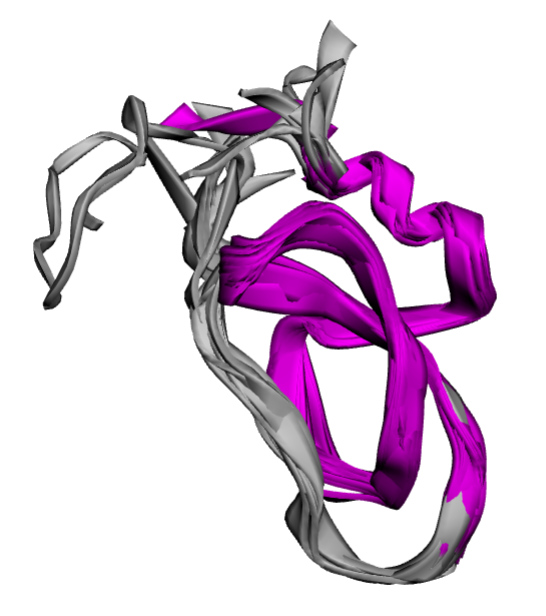
\includegraphics[width=\textwidth]{images/msa1.png}
        \caption{}
    \end{subfigure}
    \hfill
    \begin{subfigure}[t]{0.30\textwidth} 
        \centering
        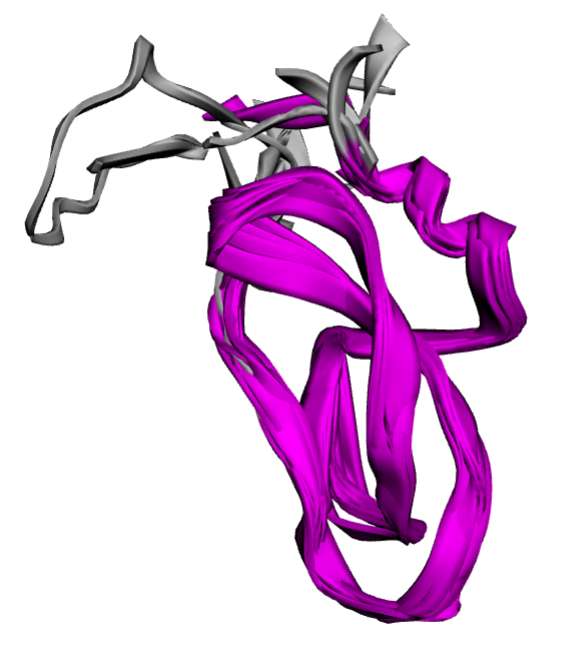
\includegraphics[width=\textwidth]{images/msa2.png} 
        \caption{}
    \end{subfigure}
    \hfill
    \begin{subfigure}[t]{0.30\textwidth} 
        \centering
        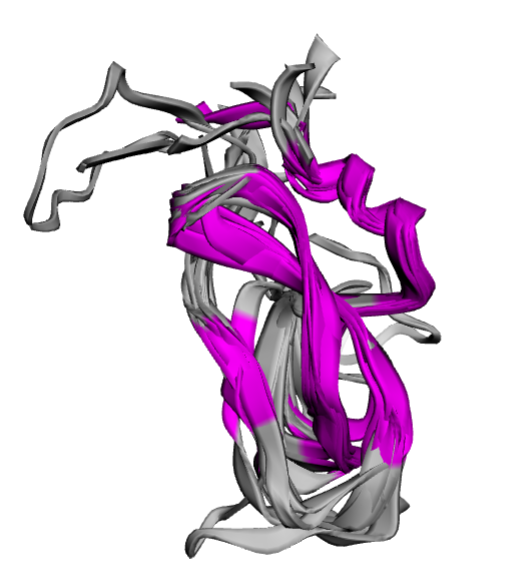
\includegraphics[width=\textwidth]{images/msa_false_negative.png} 
        \caption{}
    \end{subfigure}
    \caption{\textbf{3D representation of the multiple structures alignment with mTM-align2.} (a) represents the MSA obtained with all 12 strcutres remained after the clustering procedure, while on the (b) represent the one made with the best 10 structures selected for train the hidden markov model. (c) represent the structural alignment of the 10 structures used to build the model and 4 false negatives (the one investigated to explain the misclassification); it can be seen that the core region hilighted in purple is clearly reduced when we introduce also the false negative, meanng that they diverge in structures with respect the one represented by our model.}
    \label{fig:msa_structures}
\end{figure}

\begin{figure}[H]
    \centering
    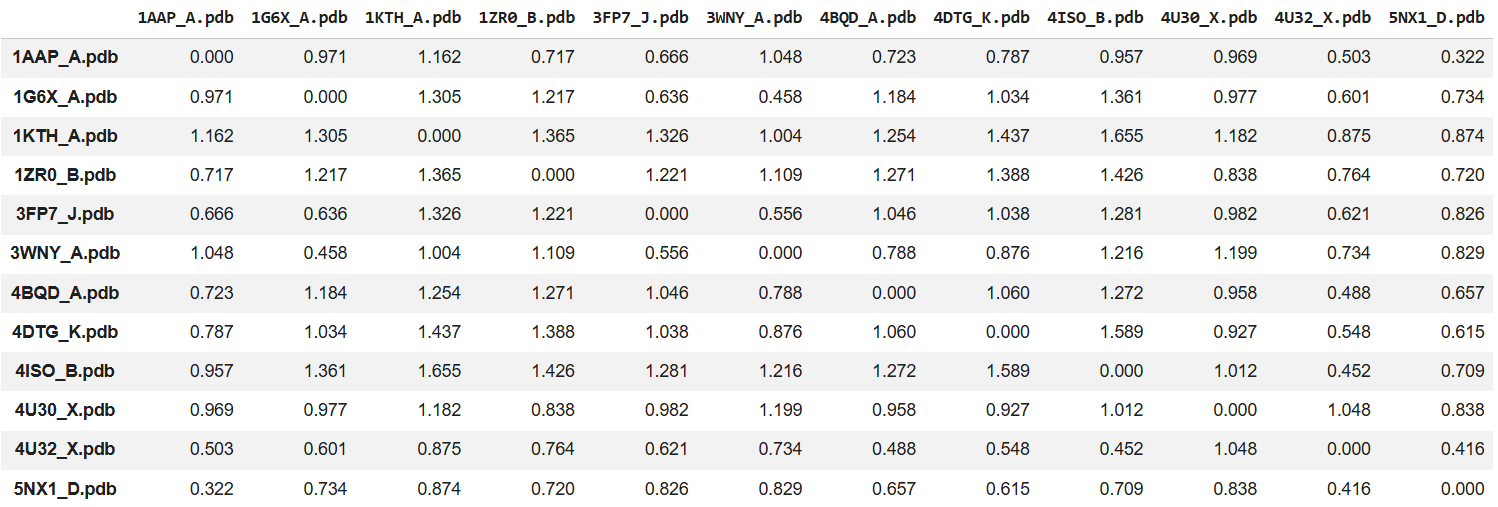
\includegraphics[width=\linewidth]{images/rmsd_table1.png}
    \caption{\textbf{Table with pairwise RMSD scores for the first MSA} (the one with all 12 structures obtained after the clustering). I used a python script to evaluate which structures has an average RMSD higher than the global average RMSD plus one standard deviation, and I obtain as result the two structures 1KTH:A and 4ISO:B (with respectivelly 1.221727 and 1.175455 as average RMSD). 
    Both 1KTH:A and 4ISO:B have an higher average RMSD but looking to the RMSD table we can see that the higher pairwise RMSD values are with specific structures, not with all. This means that their 3D structure diverges just with soem particular structures and not globally. For this reason I decide to keep them in the set of structures used to build the hidden markov model.}
    \label{fig:rmsd_table1}
\end{figure}

\begin{figure}[H]
    \centering
    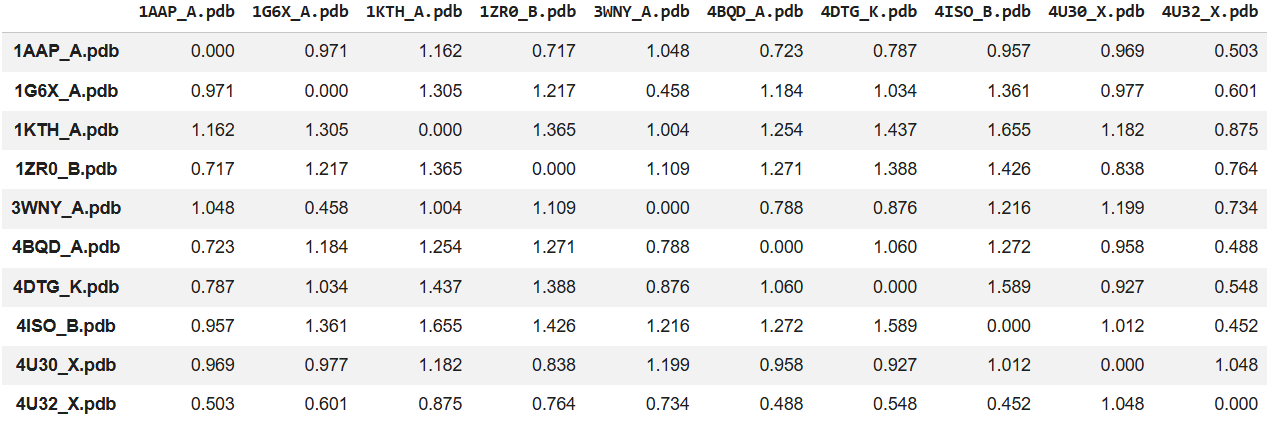
\includegraphics[width=\linewidth]{images/rmsd_table2.png}
    \caption{\textbf{Table with pairwise RMSD scores for the second MSA} (the one with just the 10 best strcutres used to build the hidden markov model). By using the same python script that evaluates which structures has an average RMSD higher than the global average RMSD plus one standard deviation, i obtain as result the same two structures as before (1KTH:A and 4ISO:B). For the same reasoning explained in the caption of the previous image, I decide to keep them.}
    \label{fig:rmsd_table2}
\end{figure}

\begin{figure}[H]
    \centering
    \begin{subfigure}[t]{\textwidth}
        \centering
        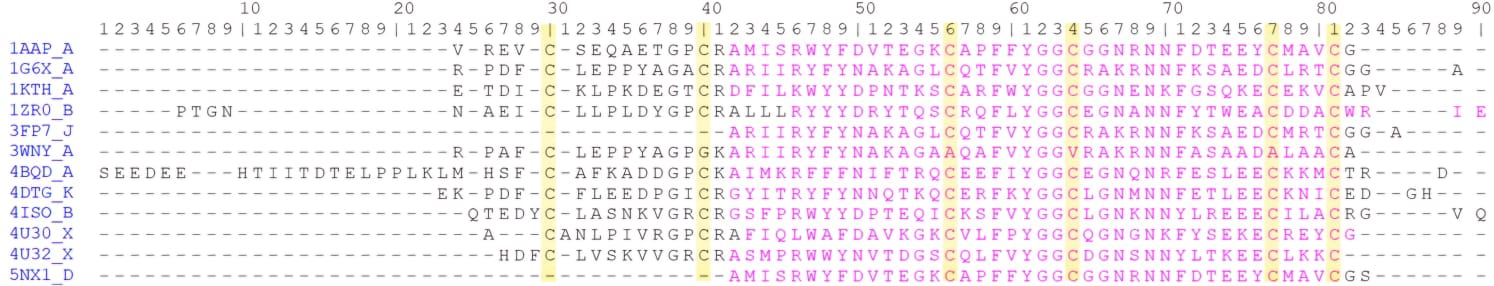
\includegraphics[width=\textwidth]{images/msa_sequences_1.jpeg}
        \caption{}
    \end{subfigure}
    \\
    \begin{subfigure}[t]{\textwidth} 
        \centering
        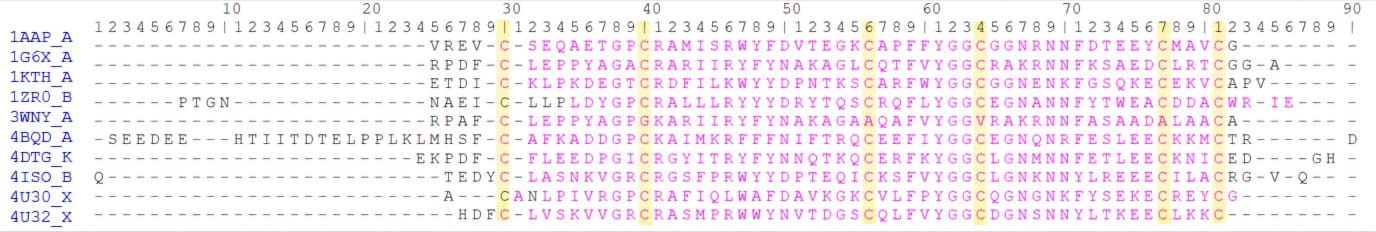
\includegraphics[width=\textwidth]{images/msa_sequences_2.jpeg} 
        \caption{}
    \end{subfigure}
    \caption{\textbf{Multiple sequence alignment obtained from multiple structure aligment with mTM-align2.} The first alignment is made with all 12 structures remained after the clustering procedure, while the second alignment show only the sequences of the best 10 structures selected for train the hidden markov model. The pink region shows the common core (most similar region with lowest RMSD across structures). The columns highlighted in yellow are the one corresponding to the six cysteines.}
    \label{fig:msa_sequences}
\end{figure}

\begin{figure}[H]
    \centering
    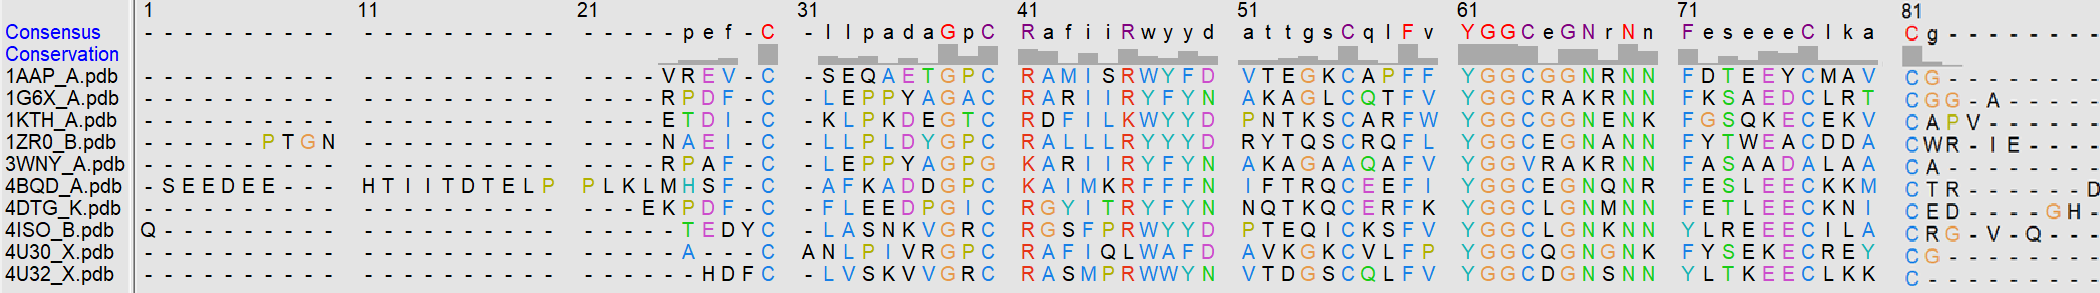
\includegraphics[width=\linewidth]{images/multiple_sequence_alignment_chimera.png}
    \caption{\textbf{Different representation of the multiple sequence alignment obtained from multiple structure aligment.} The conservation level in each position of the alignment is represented as grey bargraph.}
    \label{fig:msa_sequences_chimera}
\end{figure}

\begin{figure}[H]
    \centering
    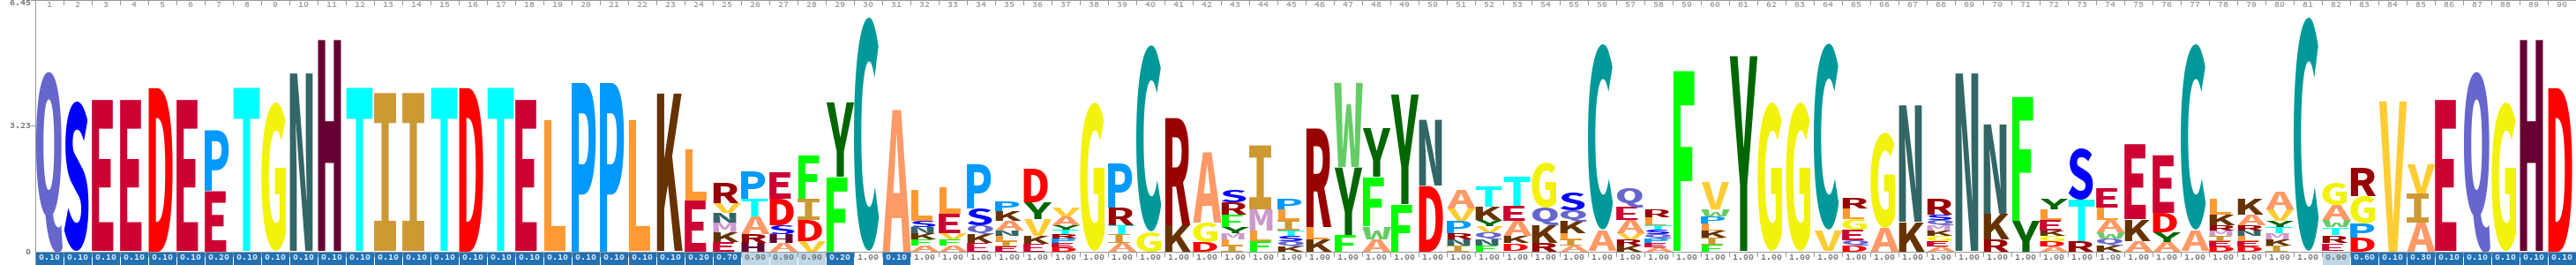
\includegraphics[width=\linewidth]{images/sequence_logo_msa.png}
    \caption{\textbf{Sequence logo of the multiple sequence alignment used to train the hidden markov model.} It was generated by using the Skylign tool. Notice that all the sixt cysteines are almost entirelly conserved.}
    \label{fig:sequence_logo_msa}
\end{figure}

\begin{figure}[H]
    \centering
    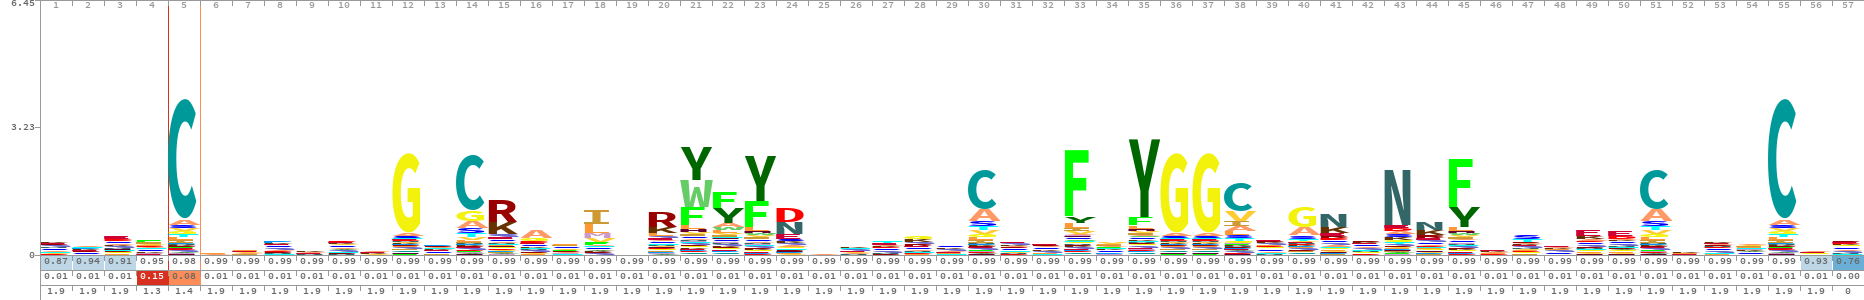
\includegraphics[width=\linewidth]{images/sequence_logo_hmm.png}
    \caption{\textbf{Sequence logo of the trained hidden markov model.} It was generated by using the Skylign tool and it represent the emission probabilities of each maching state. Notice that the sixt cysteines are still well conserved.}
    \label{fig:sequence_logo_hmm}
\end{figure}

\begin{figure}[H]
    \centering
        \begin{subfigure}[t]{\textwidth} 
        \centering
        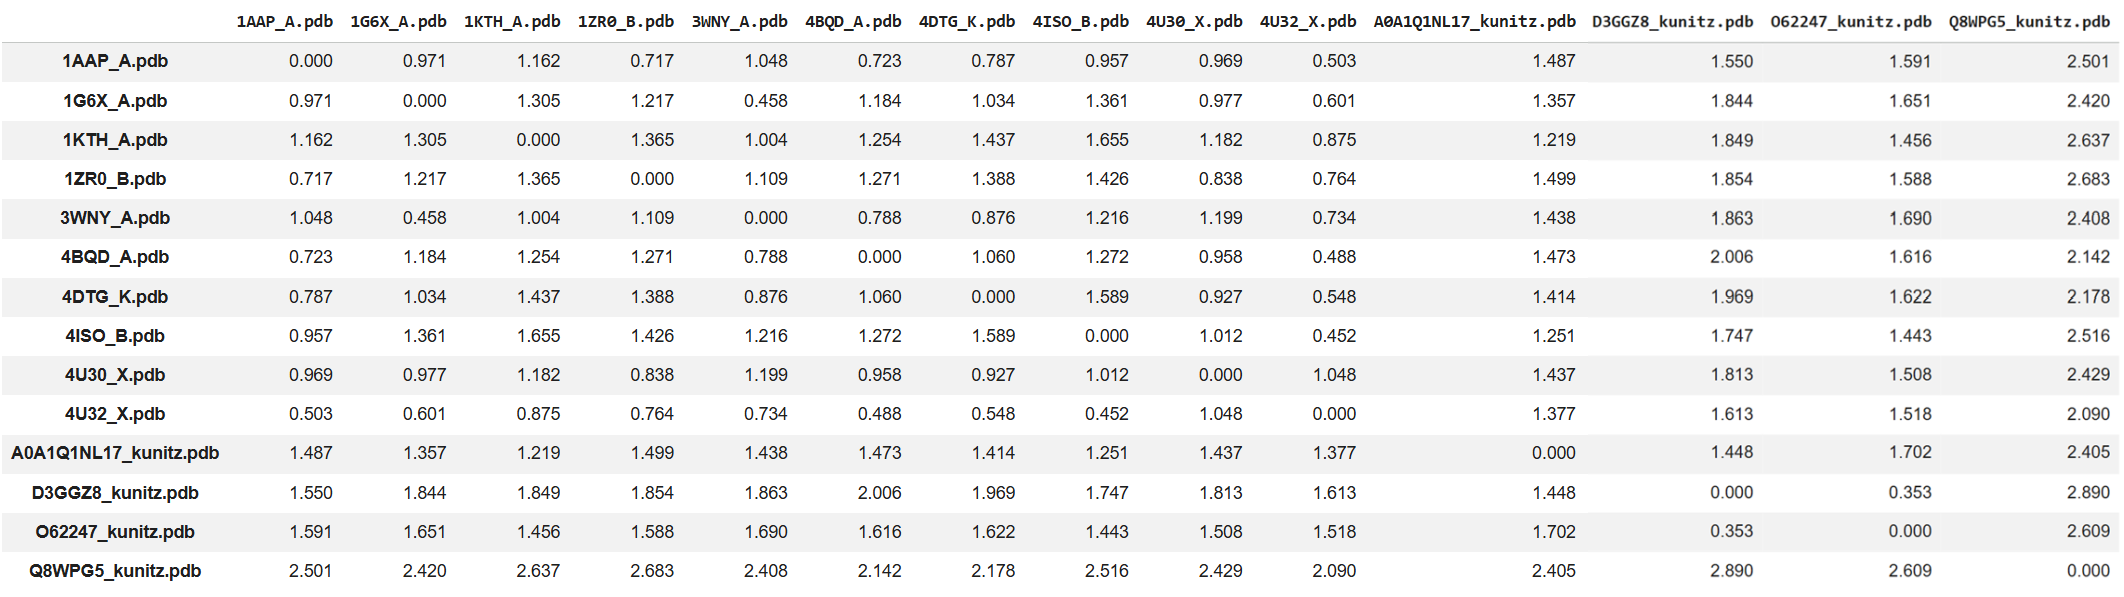
\includegraphics[width=\linewidth]{images/rmsd_table_false_negative.png}
        \caption{}
        \end{subfigure}
    \\
    \begin{subfigure}[t]{\textwidth} 
        \centering
        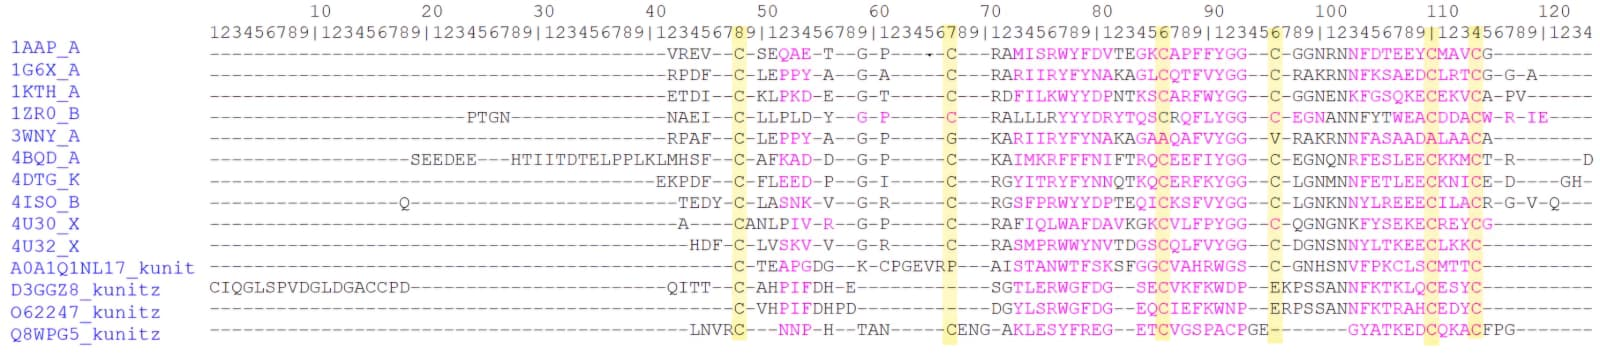
\includegraphics[width=\textwidth]{images/msa_sequences_false_negative.jpeg} 
        \caption{}
    \end{subfigure}
    \caption{\textbf{False negatives analysis based on MSA.} Table in (a) represents the RMSD value obtained from the alignment 
    of the 10 structures used to build the hidden markov model and the 4 false negative investigated in the last part of the project. (b) 
    represent the sequences alignment obtained from the structural alignment, with core region hilighted in purple and the six cisteines 
    hilighted in yellow.}
    \label{fig:false_negative}
\end{figure}

\begin{itemize}
    \item \textbf{Q8WPG5} has higher RMSD values with respect structures used to train the model (2.1-2.9 \AA), and it does not have the fourth 
    cysteine (half of the disulfide bridge C2-C4); this high structural divergence with atypical cirteines pattern suggests a very divergent 
    variant of Kunitz domain (potentially a remote homologue).
    \item \textbf{A0A1Q1NL17} RMSD versus training set in average (1.2-1.5 \AA) but it does 
    not have the second cysteine; it can be an atypical Kunitz domain not well represente in the training set. 
    \item \textbf{D3GGZ8 and O62247} are 
    the most extreme cases with e-value 0.14 and 0.012; their kunitz domain is positioned away from the N-terminus and, since they are long 
    proteins (195 and 202 aa), this penalizes e-value due to sequence length; they have high RMSD compared to the training set (1.5-1.9 \AA) 
    but very low between them (0.353 \AA); both of them do not have the second and fourth cysteines (lack of the central C2-C4 disulfide bridge); 
    finally they both belong to nematodes (organisms evolutionarily distant from vertebrates in the training set); these elements together 
    suggest that they belong to an evolutionarily divergent variation of the Kunitz domain, not well represented in the training set build 
    predominantly on vertebrates.
\end{itemize}

\end{document}